\documentclass[a4paper, 14pt]{article}
\usepackage{graphicx}
\usepackage{fancyhdr}
\usepackage{amssymb}
\usepackage{hyperref}
\newcommand{\HRule}{\rule{\linewidth}{0.5mm}}
\pagestyle{fancy}
\lhead{{\bf Parallel Programming}\\SS 2013, J. Sch\"onherr}
\rhead{Assignmen 2}
\renewcommand{\headrulewidth}{0.4pt}
\begin{document}
\begin{titlepage}
\begin{center}
\vfill
\textsc{\LARGE Parallel Programming}\\[1.5cm]
\textsc{\Large }\\[0.5cm]

\HRule \\[0.4cm]
{\huge \bfseries Assignment 2}\\[0.4cm]
\HRule \\[1.5cm]
\begin{minipage}{0.4\textwidth}
\begin{flushleft} \large
\emph{Group Members:}\\
Xugang \textsc{Zhou} 352032\\
Fangzhou \textsc{Yang} 352040
\end{flushleft}
\end{minipage}
\begin{minipage}{0.4\textwidth}
\begin{flushright} \large
\emph{Lecturer:} \\
Jan \textsc{Sch\"onherr}\\
\end{flushright}
\end{minipage}
\vfill
{\large \today}\\
\end{center}
\end{titlepage}
\thispagestyle{fancy}

\section{Exercise 1 - Sequential Overspecification}
\begin{enumerate}
\item{(a)} The sequential algorithm written does the job to commpute
  the max sub-array sum of an array of integer numbers. After running
  the code, the max sub-array sum of the integer array $a[N]$ would be
  stored in $max\_sum$.
\item{(b)} For an array of size $N$, we can derived a $O(log P + N/P)$ time
  parallel algorithm. (Suppose that P is the number of processes that
  we can run). For convinent, let's assume that P is some power of 2
  ($P = 2^n$ for $n \in \mathbb{N}$). Here's the general runnning
  algorithm:\\
\begin{verbatim}

main(num_array, N, P)
   for each sub_array in length N/P:
       sub_array.left_max =  max_sum of the array starting from the left
       sub_array.right_max = max_sum of the array starting from the right
       sub_array.max_sum = max_sum of sub_array
   for i from 1 to Log(P)
       merge the sub_array[2 * i] and sub_array[2 * i + 1] to
         merged_array using max_sum_kernel(see below)
       Set the merged_array as the new sub_arrays
   result stored in the last sub_array.max_sum
\end{verbatim}
Here's the kernel operation of
  each process.\\
\begin{verbatim}
max_sum_kernel(sub_array1, sub_array2, merged_array
   merged_array.left_max = sub_array1.left_max
   merged_arrat.right_max = sub_array2.right_max
   mergeg_array.max_sum = max(sub_array1.max_sum, sub_array2.max_sum,
                               sub_array1.right_max+sub_array2.left_max)
\end{verbatim}
\end{enumerate}

\section{Exercise 2 - Conway's Game of Life}
\begin{enumerate}
\item{a. Problem Decomposition}\\
Here we take the viriant A --Regular Parallelism. We decompose the problem by dividing the coordinate axis y to equal parts. The details of our method by Foster's Design Methodology are as follows: \\
\begin{itemize}
\item{1. Partitioning} We divide the data into small parts according to their y axis's coordinate, so that they can be parallel processed. Each part will calculate the number of neighbors for each points. The inner points, which don't stand on the boundary of the area, can be calculated at first because they are independent of other divided parts.
\item{2. Communication} Each small parts should communicate with each other to excahnge the information of the points on the boundary, because the next status of the points on the bounday depend on the points of the neighbors' boundary, too. So for each iteration of the game time, different parts will send the status of the points on the boundary to their neighbors.
\item{3. Agglomeration} By this step we group the primitive tasks to a larger task to reduce dependencies and overhead. Here we just need simply divide the primitive  matrix to submatrices equally, so that they can be mapped into each process. \\
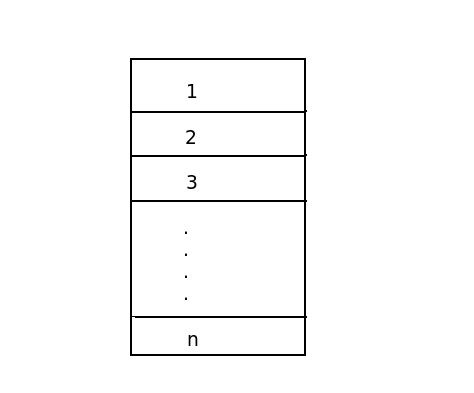
\includegraphics[width=6cm]{conway.png}
\\
To get the result of the game at time T, we just need joint all divided parts together by printing the result of each small parts sequentially. 
\item{4. Mapping} Each node processes one submatrix.
\end{itemize}

This strategy is good for the situation, that the live dots are well-distributed in the coordinate system. Otherwise, the most computation might be only concentrated on a few nodes.
Besides, the data structure of variant A is also good for the situation with high density live dots.

\item{b. Implementation} \\
The source code is in the file conway.c \\
The usage is as follows: \\
$>$mpicc.openmpi -Wall -o conway conway.c \\
$>$ccsalloc -n $<nr>$ openmpi -- ./conway $<par-NUM> <Iteration> <xNUM> <yNUM> <dotsNUM> <x1> <y1>....<xn> <yn>$ \\
$<par-NUM>$ is the number of parallel processes, which should be the same with the parameter of -n $<nr>$\\
$<Iteration>$ is the iteration times of the game.\\
$<xNUM>$ is the maximum value of the x-axis.\\
$<yNUM>$ is the maximum value of the y-axis.\\
$<dotsNUM>$ is the number of the live dots at the beginning as the input.\\
$<x1>$ $<y1>$.. are the coordinates of the living dots. They are located like: array[y1][x1]. \\
The following is the result of the \href{http://www.conwaylife.com/wiki/Pulsar}{"Pulsar"}, which is the fourth most common oscillator of Conway's Game of Life. \\
\\
>ccsalloc -n 5 openmpi -- ./conway 5 10 15 15 48 3 1 4 1 5 1 9 1 10 1 11 1 1 3 6 3 8 3 13 3 1 4 6 4 8 4 13 4 1 5 6 5 8 5 13 5 3 6 4 6 5 6 9 6 10 6 11 6 3 8 4 8 5 8 9 8 10 8 11 8 3 13 4 13 5 13 9 13 10 13 11 13 1 9 6 9 8 9 13 9 1 10 6 10 8 10 13 10 1 11 6 11 8 11 13 11
\\ 
\texttt{
initializing game...\\
initializing game...\\
initializing game...\\
initializing game...\\
initializing game...\\
map initialization done!\\
map initialization done!\\
map initialization done!\\
map initialization done!\\
map initialization done!\\
 0  0  0  0  0  0  0  0  0  0  0  0  0  0  0 \\
 0  0  0  1  1  1  0  0  0  1  1  1  0  0  0 \\
 0  0  0  0  0  0  0  0  0  0  0  0  0  0  0 \\
 0  1  0  0  0  0  1  0  1  0  0  0  0  1  0 \\
 0  1  0  0  0  0  1  0  1  0  0  0  0  1  0 \\
 0  1  0  0  0  0  1  0  1  0  0  0  0  1  0 \\
 0  0  0  1  1  1  0  0  0  1  1  1  0  0  0 \\
 0  0  0  0  0  0  0  0  0  0  0  0  0  0  0 \\
 0  0  0  1  1  1  0  0  0  1  1  1  0  0  0 \\
 0  1  0  0  0  0  1  0  1  0  0  0  0  1  0 \\
 0  1  0  0  0  0  1  0  1  0  0  0  0  1  0 \\
 0  1  0  0  0  0  1  0  1  0  0  0  0  1  0 \\
 0  0  0  0  0  0  0  0  0  0  0  0  0  0  0 \\
 0  0  0  1  1  1  0  0  0  1  1  1  0  0  0 \\
 0  0  0  0  0  0  0  0  0  0  0  0  0  0  0 \\
iteration = 1 ..\\
 -  -  -  -  X  -  -  -  -  -  X  -  -  -  - 	line: 0\\
 -  -  -  -  X  -  -  -  -  -  X  -  -  -  - 	line: 1\\
 -  -  -  -  X  X  -  -  -  X  X  -  -  -  - 	line: 2\\
 -  -  -  -  -  -  -  -  -  -  -  -  -  -  - 	line: 3\\
 X  X  X  -  -  X  X  -  X  X  -  -  X  X  X 	line: 4\\
 -  -  X  -  X  -  X  -  X  -  X  -  X  -  - 	line: 5\\
 -  -  -  -  X  X  -  -  -  X  X  -  -  -  - 	line: 6\\
 -  -  -  -  -  -  -  -  -  -  -  -  -  -  - 	line: 7\\
 -  -  -  -  X  X  -  -  -  X  X  -  -  -  - 	line: 8\\
 -  -  X  -  X  -  X  -  X  -  X  -  X  -  - 	line: 9\\
 X  X  X  -  -  X  X  -  X  X  -  -  X  X  X 	line: 10\\
 -  -  -  -  -  -  -  -  -  -  -  -  -  -  - 	line: 11\\
 -  -  -  -  X  X  -  -  -  X  X  -  -  -  - 	line: 12\\
 -  -  -  -  X  -  -  -  -  -  X  -  -  -  - 	line: 13\\
 -  -  -  -  X  -  -  -  -  -  X  -  -  -  - 	line: 14\\
\newpage
iteration = 2 ..\\
 -  -  -  -  -  -  -  -  -  -  -  -  -  -  - 	line: 0\\
 -  -  -  X  X  -  -  -  -  -  X  X  -  -  - 	line: 1\\
 -  -  -  -  X  X  -  -  -  X  X  -  -  -  - 	line: 2\\
 -  X  -  -  X  -  X  -  X  -  X  -  -  X  - 	line: 3\\
 -  X  X  X  -  X  X  -  X  X  -  X  X  X  - 	line: 4\\
 -  -  X  -  X  -  X  -  X  -  X  -  X  -  - 	line: 5\\
 -  -  -  X  X  X  -  -  -  X  X  X  -  -  - 	line: 6\\
 -  -  -  -  -  -  -  -  -  -  -  -  -  -  - 	line: 7\\
 -  -  -  X  X  X  -  -  -  X  X  X  -  -  - 	line: 8\\
 -  -  X  -  X  -  X  -  X  -  X  -  X  -  - 	line: 9\\
 -  X  X  X  -  X  X  -  X  X  -  X  X  X  - 	line: 10\\
 -  X  -  -  X  -  X  -  X  -  X  -  -  X  - 	line: 11\\
 -  -  -  -  X  X  -  -  -  X  X  -  -  -  - 	line: 12\\
 -  -  -  X  X  -  -  -  -  -  X  X  -  -  - 	line: 13\\
 -  -  -  -  -  -  -  -  -  -  -  -  -  -  - 	line: 14\\
iteration = 3 ..\\
 -  -  -  -  -  -  -  -  -  -  -  -  -  -  - 	line: 0\\
 -  -  -  X  X  X  -  -  -  X  X  X  -  -  - 	line: 1\\
 -  -  -  -  -  -  -  -  -  -  -  -  -  -  - 	line: 2\\
 -  X  -  -  -  -  X  -  X  -  -  -  -  X  - 	line: 3\\
 -  X  -  -  -  -  X  -  X  -  -  -  -  X  - 	line: 4\\
 -  X  -  -  -  -  X  -  X  -  -  -  -  X  - 	line: 5\\
 -  -  -  X  X  X  -  -  -  X  X  X  -  -  - 	line: 6\\
 -  -  -  -  -  -  -  -  -  -  -  -  -  -  - 	line: 7\\
 -  -  -  X  X  X  -  -  -  X  X  X  -  -  - 	line: 8\\
 -  X  -  -  -  -  X  -  X  -  -  -  -  X  - 	line: 9\\
 -  X  -  -  -  -  X  -  X  -  -  -  -  X  - 	line: 10\\
 -  X  -  -  -  -  X  -  X  -  -  -  -  X  - 	line: 11\\
 -  -  -  -  -  -  -  -  -  -  -  -  -  -  - 	line: 12\\
 -  -  -  X  X  X  -  -  -  X  X  X  -  -  - 	line: 13\\
 -  -  -  -  -  -  -  -  -  -  -  -  -  -  - 	line: 14\\
iteration = 4 ..\\
 -  -  -  -  X  -  -  -  -  -  X  -  -  -  - 	line: 0\\
 -  -  -  -  X  -  -  -  -  -  X  -  -  -  - 	line: 1\\
 -  -  -  -  X  X  -  -  -  X  X  -  -  -  - 	line: 2\\
 -  -  -  -  -  -  -  -  -  -  -  -  -  -  - 	line: 3\\
 X  X  X  -  -  X  X  -  X  X  -  -  X  X  X 	line: 4\\
 -  -  X  -  X  -  X  -  X  -  X  -  X  -  - 	line: 5\\
 -  -  -  -  X  X  -  -  -  X  X  -  -  -  - 	line: 6\\
 -  -  -  -  -  -  -  -  -  -  -  -  -  -  - 	line: 7\\
 -  -  -  -  X  X  -  -  -  X  X  -  -  -  - 	line: 8\\
 -  -  X  -  X  -  X  -  X  -  X  -  X  -  - 	line: 9\\
 X  X  X  -  -  X  X  -  X  X  -  -  X  X  X 	line: 10\\
 -  -  -  -  -  -  -  -  -  -  -  -  -  -  - 	line: 11\\
 -  -  -  -  X  X  -  -  -  X  X  -  -  -  - 	line: 12\\
 -  -  -  -  X  -  -  -  -  -  X  -  -  -  - 	line: 13\\
 -  -  -  -  X  -  -  -  -  -  X  -  -  -  - 	line: 14\\
\newpage
iteration = 5 ..\\
 -  -  -  -  -  -  -  -  -  -  -  -  -  -  - 	line: 0\\
 -  -  -  X  X  -  -  -  -  -  X  X  -  -  - 	line: 1\\
 -  -  -  -  X  X  -  -  -  X  X  -  -  -  - 	line: 2\\
 -  X  -  -  X  -  X  -  X  -  X  -  -  X  - 	line: 3\\
 -  X  X  X  -  X  X  -  X  X  -  X  X  X  - 	line: 4\\
 -  -  X  -  X  -  X  -  X  -  X  -  X  -  - 	line: 5\\
 -  -  -  X  X  X  -  -  -  X  X  X  -  -  - 	line: 6\\
 -  -  -  -  -  -  -  -  -  -  -  -  -  -  - 	line: 7\\
 -  -  -  X  X  X  -  -  -  X  X  X  -  -  - 	line: 8\\
 -  -  X  -  X  -  X  -  X  -  X  -  X  -  - 	line: 9\\
 -  X  X  X  -  X  X  -  X  X  -  X  X  X  - 	line: 10\\
 -  X  -  -  X  -  X  -  X  -  X  -  -  X  - 	line: 11\\
 -  -  -  -  X  X  -  -  -  X  X  -  -  -  - 	line: 12\\
 -  -  -  X  X  -  -  -  -  -  X  X  -  -  - 	line: 13\\
 -  -  -  -  -  -  -  -  -  -  -  -  -  -  - 	line: 14\\
iteration = 6 ..\\
 -  -  -  -  -  -  -  -  -  -  -  -  -  -  - 	line: 0\\
 -  -  -  X  X  X  -  -  -  X  X  X  -  -  - 	line: 1\\
 -  -  -  -  -  -  -  -  -  -  -  -  -  -  - 	line: 2\\
 -  X  -  -  -  -  X  -  X  -  -  -  -  X  - 	line: 3\\
 -  X  -  -  -  -  X  -  X  -  -  -  -  X  - 	line: 4\\
 -  X  -  -  -  -  X  -  X  -  -  -  -  X  - 	line: 5\\
 -  -  -  X  X  X  -  -  -  X  X  X  -  -  - 	line: 6\\
 -  -  -  -  -  -  -  -  -  -  -  -  -  -  - 	line: 7\\
 -  -  -  X  X  X  -  -  -  X  X  X  -  -  - 	line: 8\\
 -  X  -  -  -  -  X  -  X  -  -  -  -  X  - 	line: 9\\
 -  X  -  -  -  -  X  -  X  -  -  -  -  X  - 	line: 10\\
 -  X  -  -  -  -  X  -  X  -  -  -  -  X  - 	line: 11\\
 -  -  -  -  -  -  -  -  -  -  -  -  -  -  - 	line: 12\\
 -  -  -  X  X  X  -  -  -  X  X  X  -  -  - 	line: 13\\
 -  -  -  -  -  -  -  -  -  -  -  -  -  -  - 	line: 14\\
iteration = 7 ..\\
 -  -  -  -  X  -  -  -  -  -  X  -  -  -  - 	line: 0\\
 -  -  -  -  X  -  -  -  -  -  X  -  -  -  - 	line: 1\\
 -  -  -  -  X  X  -  -  -  X  X  -  -  -  - 	line: 2\\
 -  -  -  -  -  -  -  -  -  -  -  -  -  -  - 	line: 3\\
 X  X  X  -  -  X  X  -  X  X  -  -  X  X  X 	line: 4\\
 -  -  X  -  X  -  X  -  X  -  X  -  X  -  - 	line: 5\\
 -  -  -  -  X  X  -  -  -  X  X  -  -  -  - 	line: 6\\
 -  -  -  -  -  -  -  -  -  -  -  -  -  -  - 	line: 7\\
 -  -  -  -  X  X  -  -  -  X  X  -  -  -  - 	line: 8\\
 -  -  X  -  X  -  X  -  X  -  X  -  X  -  - 	line: 9\\
 X  X  X  -  -  X  X  -  X  X  -  -  X  X  X 	line: 10\\
 -  -  -  -  -  -  -  -  -  -  -  -  -  -  - 	line: 11\\
 -  -  -  -  X  X  -  -  -  X  X  -  -  -  - 	line: 12\\
 -  -  -  -  X  -  -  -  -  -  X  -  -  -  - 	line: 13\\
 -  -  -  -  X  -  -  -  -  -  X  -  -  -  - 	line: 14\\
\newpage
iteration = 8 ..\\
 -  -  -  -  -  -  -  -  -  -  -  -  -  -  - 	line: 0\\
 -  -  -  X  X  -  -  -  -  -  X  X  -  -  - 	line: 1\\
 -  -  -  -  X  X  -  -  -  X  X  -  -  -  - 	line: 2\\
 -  X  -  -  X  -  X  -  X  -  X  -  -  X  - 	line: 3\\
 -  X  X  X  -  X  X  -  X  X  -  X  X  X  - 	line: 4\\
 -  -  X  -  X  -  X  -  X  -  X  -  X  -  - 	line: 5\\
 -  -  -  X  X  X  -  -  -  X  X  X  -  -  - 	line: 6\\
 -  -  -  -  -  -  -  -  -  -  -  -  -  -  - 	line: 7\\
 -  -  -  X  X  X  -  -  -  X  X  X  -  -  - 	line: 8\\
 -  -  X  -  X  -  X  -  X  -  X  -  X  -  - 	line: 9\\
 -  X  X  X  -  X  X  -  X  X  -  X  X  X  - 	line: 10\\
 -  X  -  -  X  -  X  -  X  -  X  -  -  X  - 	line: 11\\
 -  -  -  -  X  X  -  -  -  X  X  -  -  -  - 	line: 12\\
 -  -  -  X  X  -  -  -  -  -  X  X  -  -  - 	line: 13\\
 -  -  -  -  -  -  -  -  -  -  -  -  -  -  - 	line: 14\\
iteration = 9 ..\\
 -  -  -  -  -  -  -  -  -  -  -  -  -  -  - 	line: 0\\
 -  -  -  X  X  X  -  -  -  X  X  X  -  -  - 	line: 1\\
 -  -  -  -  -  -  -  -  -  -  -  -  -  -  - 	line: 2\\
 -  X  -  -  -  -  X  -  X  -  -  -  -  X  - 	line: 3\\
 -  X  -  -  -  -  X  -  X  -  -  -  -  X  - 	line: 4\\
 -  X  -  -  -  -  X  -  X  -  -  -  -  X  - 	line: 5\\
 -  -  -  X  X  X  -  -  -  X  X  X  -  -  - 	line: 6\\
 -  -  -  -  -  -  -  -  -  -  -  -  -  -  - 	line: 7\\
 -  -  -  X  X  X  -  -  -  X  X  X  -  -  - 	line: 8\\
 -  X  -  -  -  -  X  -  X  -  -  -  -  X  - 	line: 9\\
 -  X  -  -  -  -  X  -  X  -  -  -  -  X  - 	line: 10\\
 -  X  -  -  -  -  X  -  X  -  -  -  -  X  - 	line: 11\\
 -  -  -  -  -  -  -  -  -  -  -  -  -  -  - 	line: 12\\
 -  -  -  X  X  X  -  -  -  X  X  X  -  -  - 	line: 13\\
 -  -  -  -  -  -  -  -  -  -  -  -  -  -  - 	line: 14\\
iteration = 10 ..\\
 -  -  -  -  X  -  -  -  -  -  X  -  -  -  - 	line: 0\\
 -  -  -  -  X  -  -  -  -  -  X  -  -  -  - 	line: 1\\
 -  -  -  -  X  X  -  -  -  X  X  -  -  -  - 	line: 2\\
 -  -  -  -  -  -  -  -  -  -  -  -  -  -  - 	line: 3\\
 X  X  X  -  -  X  X  -  X  X  -  -  X  X  X 	line: 4\\
 -  -  X  -  X  -  X  -  X  -  X  -  X  -  - 	line: 5\\
 -  -  -  -  X  X  -  -  -  X  X  -  -  -  - 	line: 6\\
 -  -  -  -  -  -  -  -  -  -  -  -  -  -  - 	line: 7\\
 -  -  -  -  X  X  -  -  -  X  X  -  -  -  - 	line: 8\\
 -  -  X  -  X  -  X  -  X  -  X  -  X  -  - 	line: 9\\
 X  X  X  -  -  X  X  -  X  X  -  -  X  X  X 	line: 10\\
 -  -  -  -  -  -  -  -  -  -  -  -  -  -  - 	line: 11\\
 -  -  -  -  X  X  -  -  -  X  X  -  -  -  - 	line: 12\\
 -  -  -  -  X  -  -  -  -  -  X  -  -  -  - 	line: 13\\
 -  -  -  -  X  -  -  -  -  -  X  -  -  -  - 	line: 14\\
runopenmpi: ./conway exited with 0\\
}
\end{enumerate}
\end{document}
